\chapter{Results and Analysis}
\label{Results:chap:chap7}
\graphicspath{{16.Chapter7/Images/}}

This chapter goes through the empirical results of FIP-FL on the grid defined in Chapter~\ref{Setup:chap:chap6}. Each table reports the relevant round-300 numbers --- overall accuracy ($\text{ACC}$), target-class accuracy ($T_{\text{acc}}$), other-label accuracy ($O_{\text{acc}}$), the true positive rate (TPR), and the false positive rate (FPR). Accuracies are quoted as percentages, and TPR and FPR are quoted as proportions in $[0,1]$.

%=====================================================================
\section{Non-IID Partition, Untargeted Attacks}
\label{sec:res-nonIID-untarg}

Of the four non-IID rows, the untargeted one is in some ways the most demanding. The label skew has already pushed the honest-client gradients away from each other, and on top of that the malicious clients are sending in label-flipped gradients that genuinely point away from the descent direction. Overall accuracy is the right utility number to read here, with TPR and FPR sitting alongside it as the cost-of-filtering pair.

\subsection{MNIST}
\label{sec:res-nonIID-untarg-mnist}

\begin{table}[H]
\centering
\caption{MNIST, non-IID partition, untargeted label-flipping attack.}
\label{tab:res-nonIID-untarg-mnist}
\begin{tabular}{@{}cccccc@{}}
\toprule
\textbf{AR} & \textbf{ACC (\%)} & \textbf{$T_{\text{acc}}$ (\%)} & \textbf{$O_{\text{acc}}$ (\%)} & \textbf{TPR} & \textbf{FPR} \\
\midrule
10\% & 91.22 & 97.60 & 90.18 & 1.00 & 0.00 \\
20\% & 91.02 & 97.87 & 89.94 & 1.00 & 0.00 \\
30\% & 90.78 & 97.33 & 89.31 & 1.00 & 0.00 \\
50\% & 91.10 & 97.51 & 89.91 & 1.00 & 0.20 \\
\bottomrule
\end{tabular}
\end{table}

\subsection{KDDCup99}
\label{sec:res-nonIID-untarg-kdd}

\begin{table}[H]
\centering
\caption{KDDCup99, non-IID partition (Dirichlet $\alpha=0.5$), untargeted label-flipping attack.}
\label{tab:res-nonIID-untarg-kdd}
\begin{tabular}{@{}cccccc@{}}
\toprule
\textbf{AR} & \textbf{ACC (\%)} & \textbf{$T_{\text{acc}}$ (\%)} & \textbf{$O_{\text{acc}}$ (\%)} & \textbf{TPR} & \textbf{FPR} \\
\midrule
10\% & 99.71 & 99.50 & 84.62 & 1.00 & 0.00 \\
20\% & 99.72 & 99.55 & 83.65 & 1.00 & 0.00 \\
30\% & 99.69 & 99.45 & 85.58 & 1.00 & 0.14 \\
50\% & 99.69 & 99.70 & 77.88 & 1.00 & 0.40 \\
\bottomrule
\end{tabular}
\end{table}

\paragraph{Observations.} Across both datasets, FIP-FL ends up rejecting every single malicious update and the utility number stays close to its undefended-clean value even under the non-IID untargeted load. On MNIST the ACC sits between $90.78\%$ and $91.22\%$, and false rejection only kicks in once the attack rate hits $50\%$. On KDDCup99 the ACC remains above $99.6\%$ throughout the sweep, even at the point where the FPR begins to rise under the heaviest non-IID setting.

\begin{figure}[!htbp]
\centering
\subfigure[MNIST ACC trajectory]{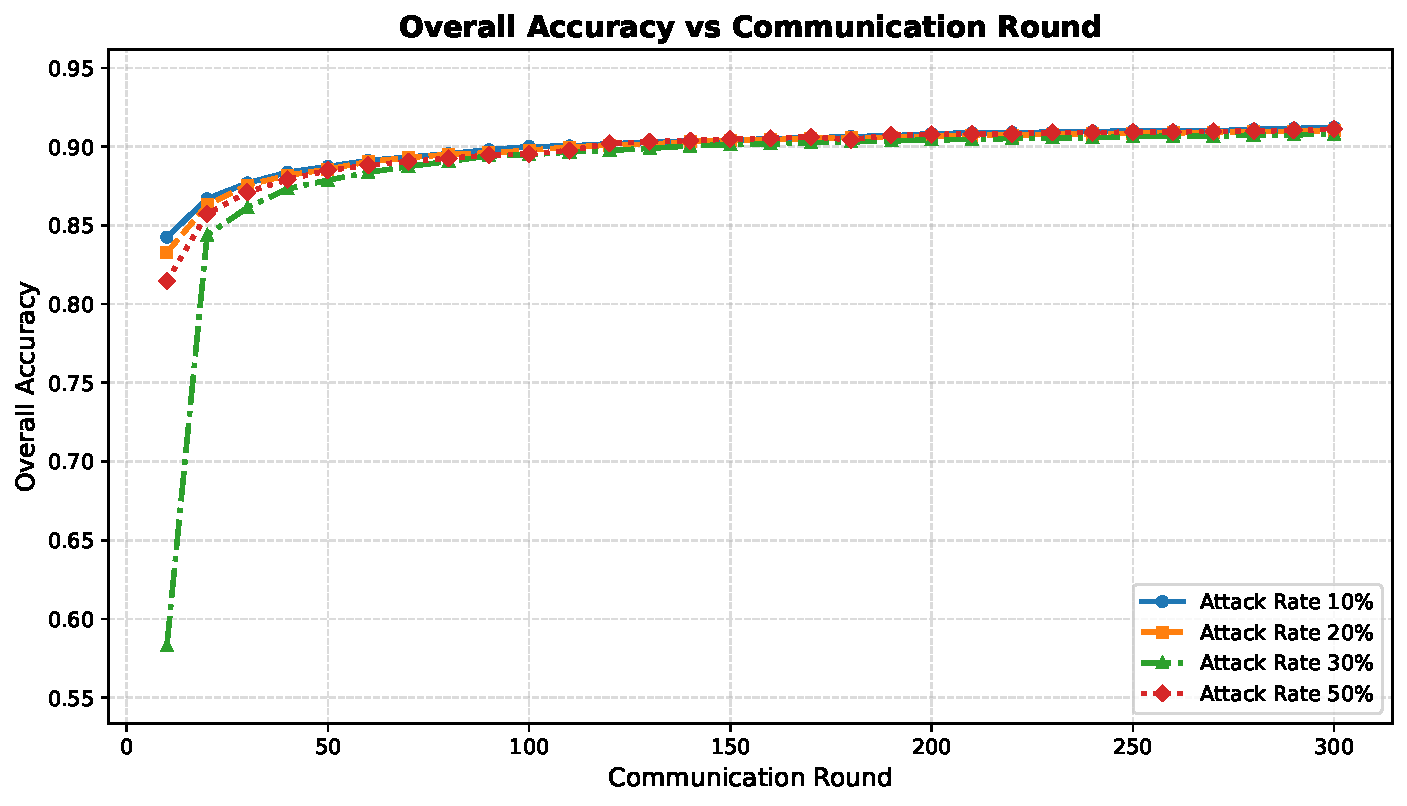
\includegraphics[width=0.47\textwidth]{fig_noniid_untargeted_mnist_acc.pdf}}
\hfill
\subfigure[KDDCup99 ACC trajectory]{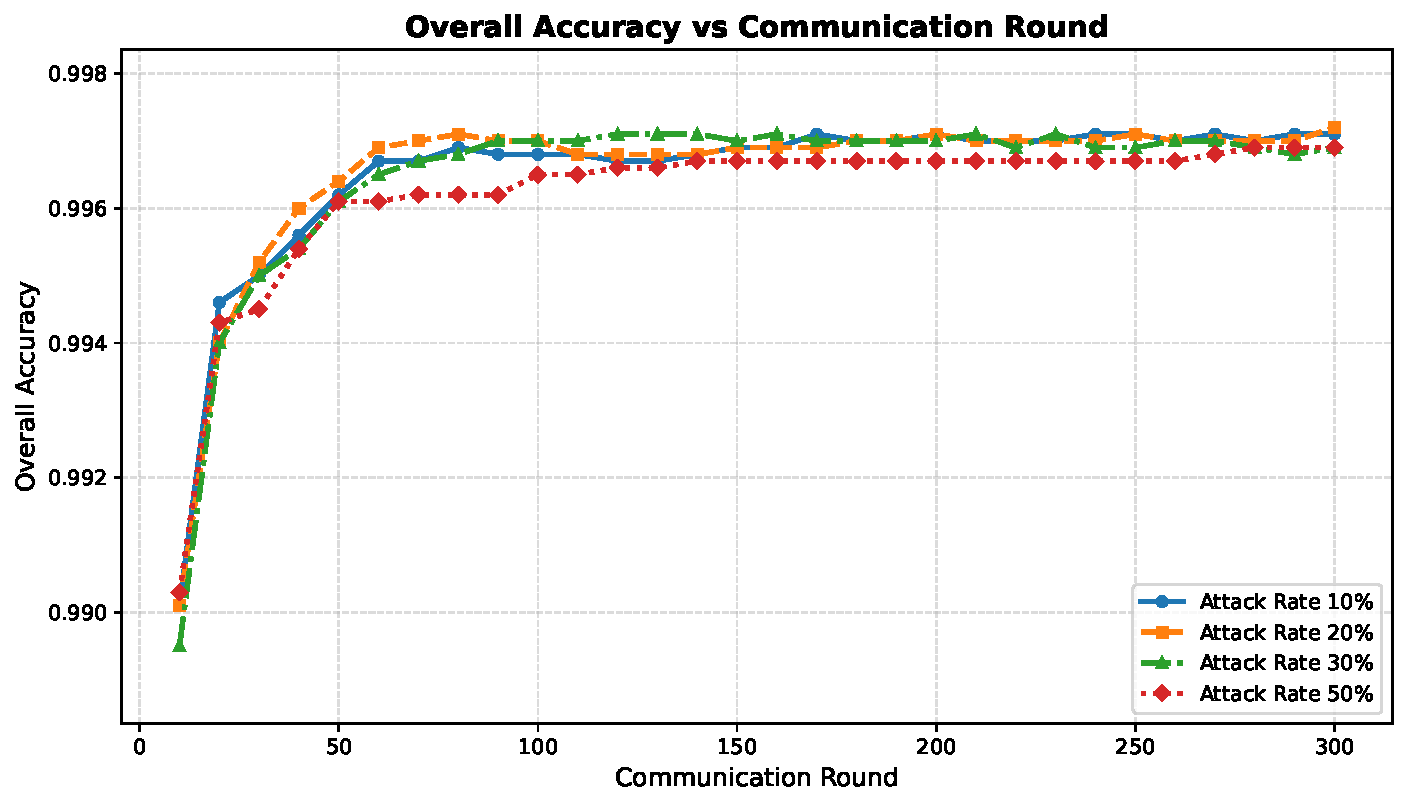
\includegraphics[width=0.47\textwidth]{fig_noniid_untargeted_kdd_acc.pdf}}
\vspace{0.4em}
\subfigure[MNIST malicious-client TPR]{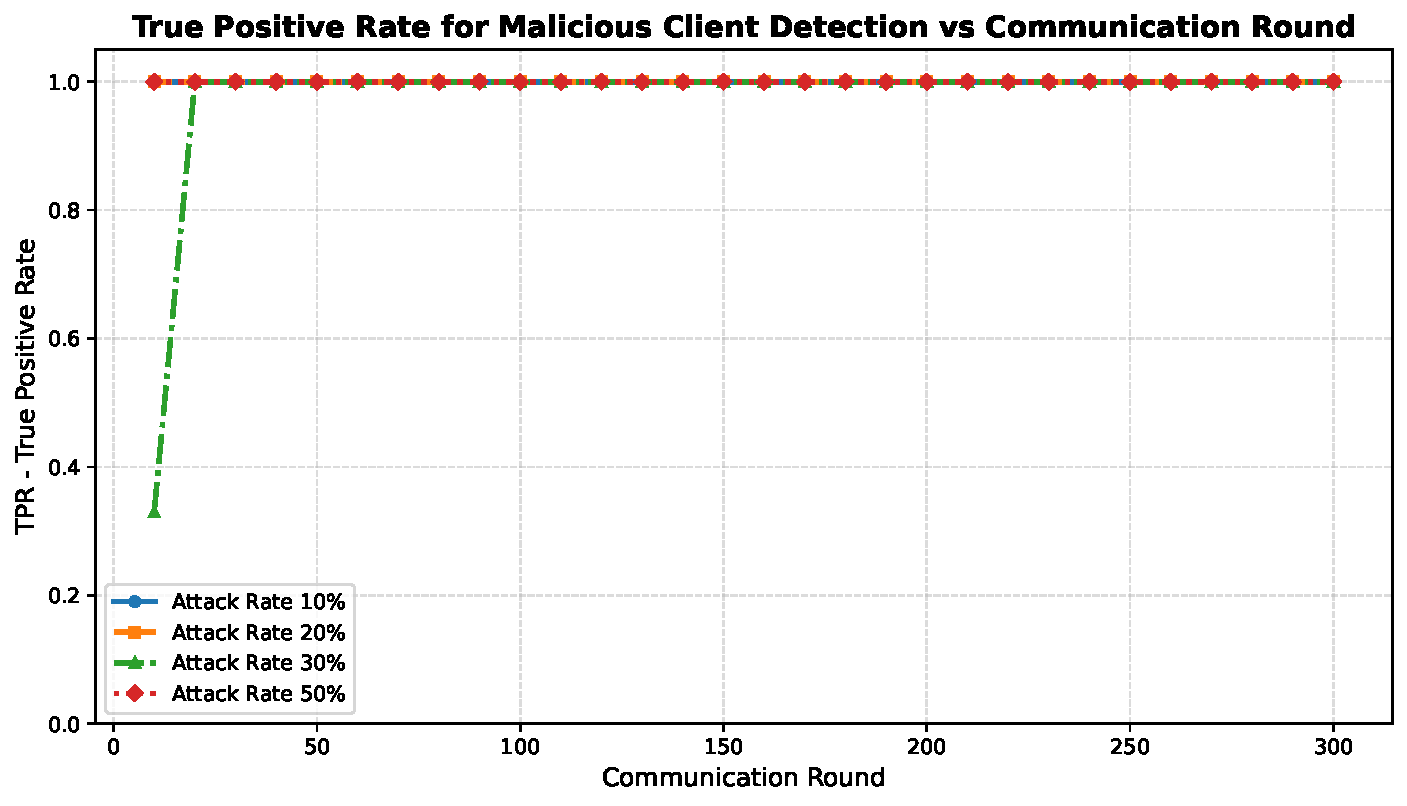
\includegraphics[width=0.47\textwidth]{fig_noniid_untargeted_mnist_tpr.pdf}}
\hfill
\subfigure[KDDCup99 malicious-client TPR]{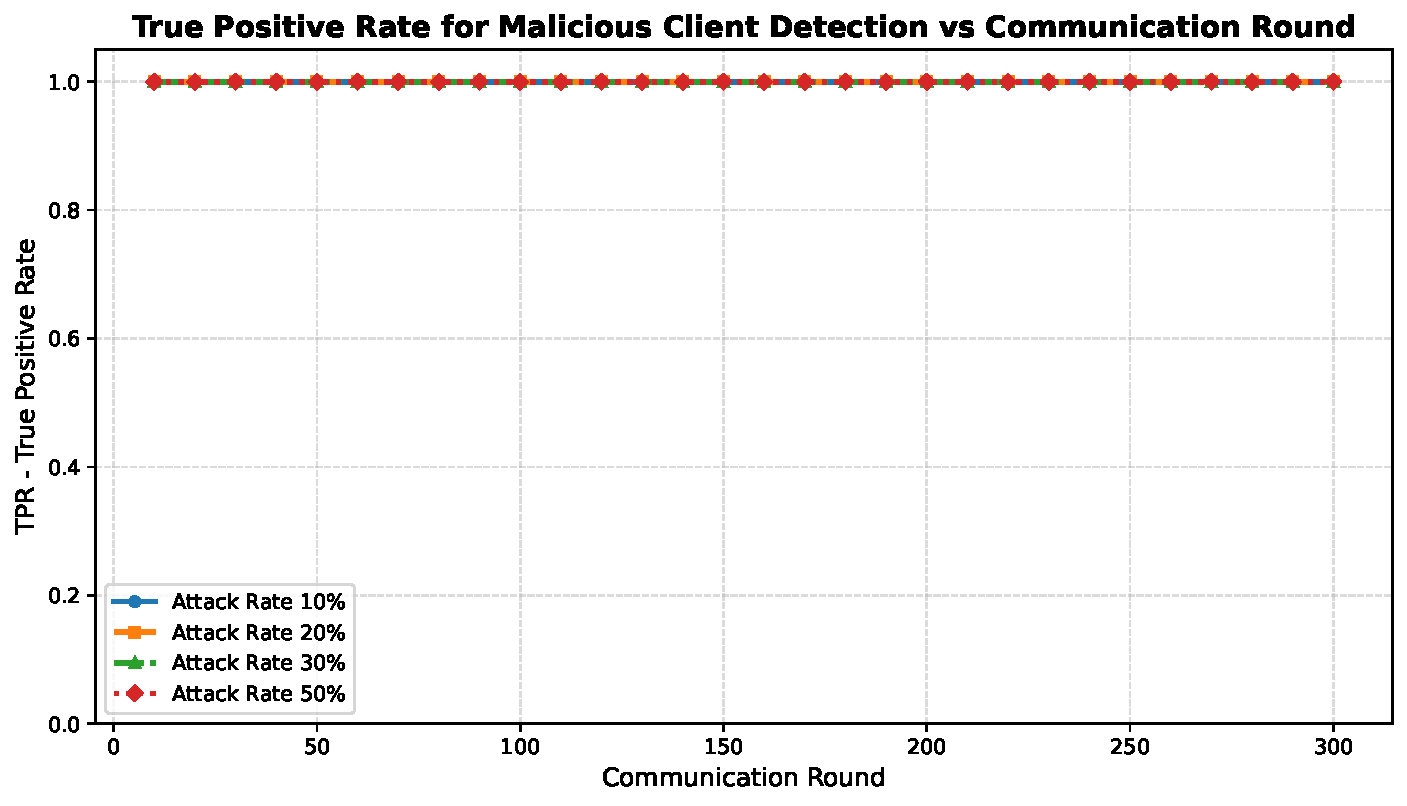
\includegraphics[width=0.47\textwidth]{fig_noniid_untargeted_kdd_tpr.pdf}}
\caption{Non-IID untargeted attack dynamics over 300 communication rounds. Accuracy converges stably for both datasets, while the direction/magnitude audit reaches perfect malicious-client detection by the final round.}
\label{fig:res-noniid-untargeted-dynamics}
\end{figure}

%=====================================================================
\section{Non-IID Partition, Targeted Attacks}
\label{sec:res-nonIID-targ}

A targeted label-flipping attack is a more delicate kind of poisoning than the untargeted case. It tries to break one specific source class while letting the global accuracy stay believable, so reading ACC alone would actively hide the damage. The number that matters here is the target-class accuracy $T_{\text{acc}}$.

\subsection{MNIST}
\label{sec:res-nonIID-targ-mnist}

\begin{table}[H]
\centering
\caption{MNIST, non-IID, targeted label-flipping attack $(c_s=0,c_t=7)$; SenSys 2026 headline targeted-accuracy cell.}
\label{tab:res-nonIID-targ-mnist}
\begin{tabular}{@{}cccc@{}}
\toprule
\textbf{AR} & \textbf{Undefended (\%)} & \textbf{Auditor-based (\%)} & \textbf{FIP-FL (\%)} \\
\midrule
50\% & $\approx 7.00$ & 96.50 & 97.69 \\
\bottomrule
\end{tabular}
\end{table}

\subsection{KDDCup99}
\label{sec:res-nonIID-targ-kdd}

\begin{table}[H]
\centering
\caption{KDDCup99, non-IID partition (2 shards/client), targeted label-flipping attack.}
\label{tab:res-nonIID-targ-kdd}
\begin{tabular}{@{}cccccc@{}}
\toprule
\textbf{AR} & \textbf{ACC (\%)} & \textbf{$T_{\text{acc}}$ (\%)} & \textbf{$O_{\text{acc}}$ (\%)} & \textbf{TPR} & \textbf{FPR} \\
\midrule
10\% & 99.54 & 99.75 & 63.46 & 1.00 & 0.00 \\
20\% & 99.69 & 99.65 & 78.85 & 1.00 & 0.00 \\
30\% & 99.70 & 99.50 & 82.69 & 1.00 & 0.00 \\
50\% & 99.52 & 98.41 & 86.54 & 1.00 & 0.00 \\
\bottomrule
\end{tabular}
\end{table}

\paragraph{Observations.} The MNIST row is the headline cell from the accepted SenSys 2026 poster. With $50\%$ of the clients turning malicious, FIP-FL pushes $T_{\text{acc}}$ from roughly $7\%$ in the undefended run all the way up to $97.69\%$ --- a number that sits above the $96.5\%$ reported by the auditor-based scheme of Yazdinejad et al.~\cite{yazdinejad2024robust}. KDDCup99 follows the same detection pattern across the full attack-rate sweep, with no false positives anywhere in the table and $T_{\text{acc}}=98.41\%$ even at the $50\%$ row.

\begin{figure}[!htbp]
\centering
\subfigure[Target-class accuracy trajectory]{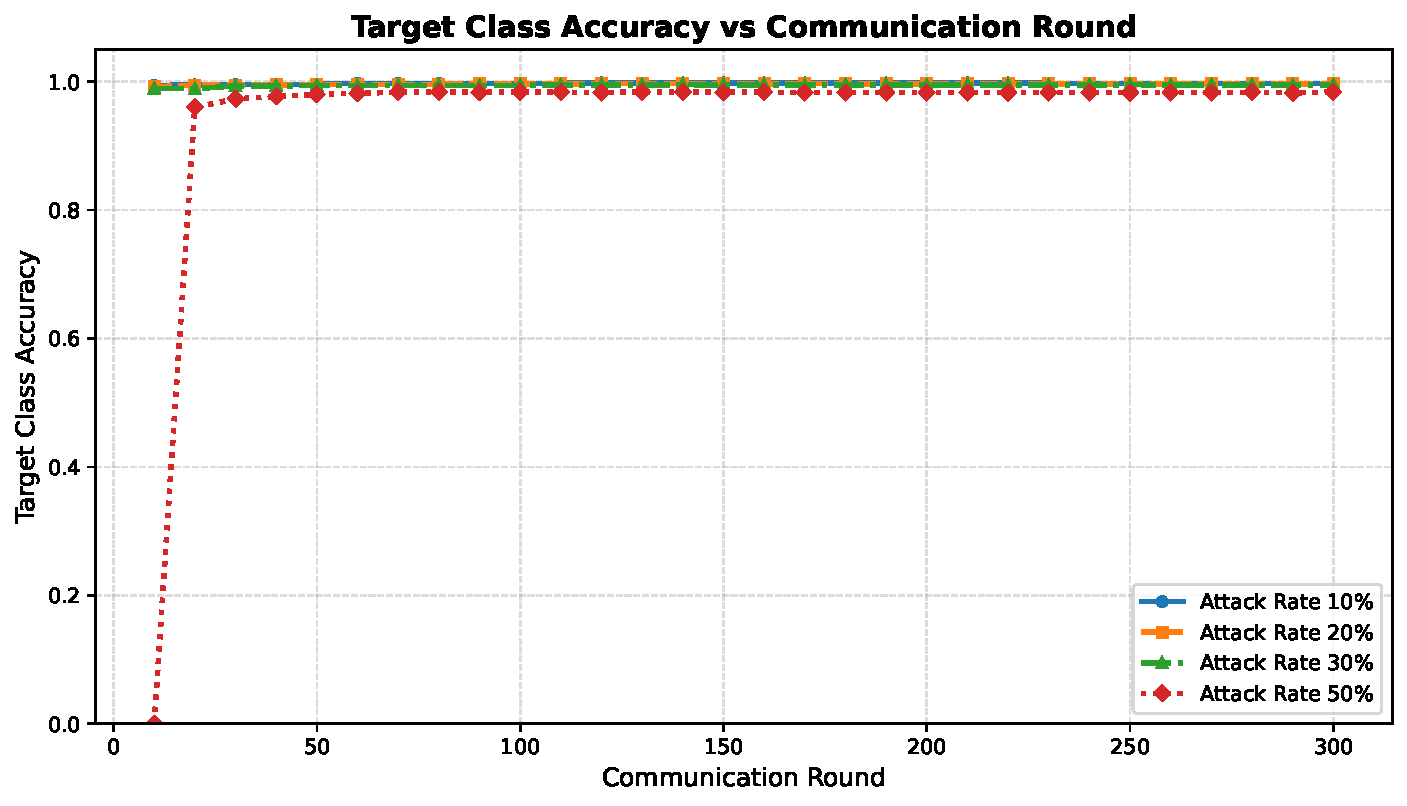
\includegraphics[width=0.47\textwidth]{fig_noniid_targeted_kdd_tacc.pdf}}
\hfill
\subfigure[Round-300 accuracy comparison]{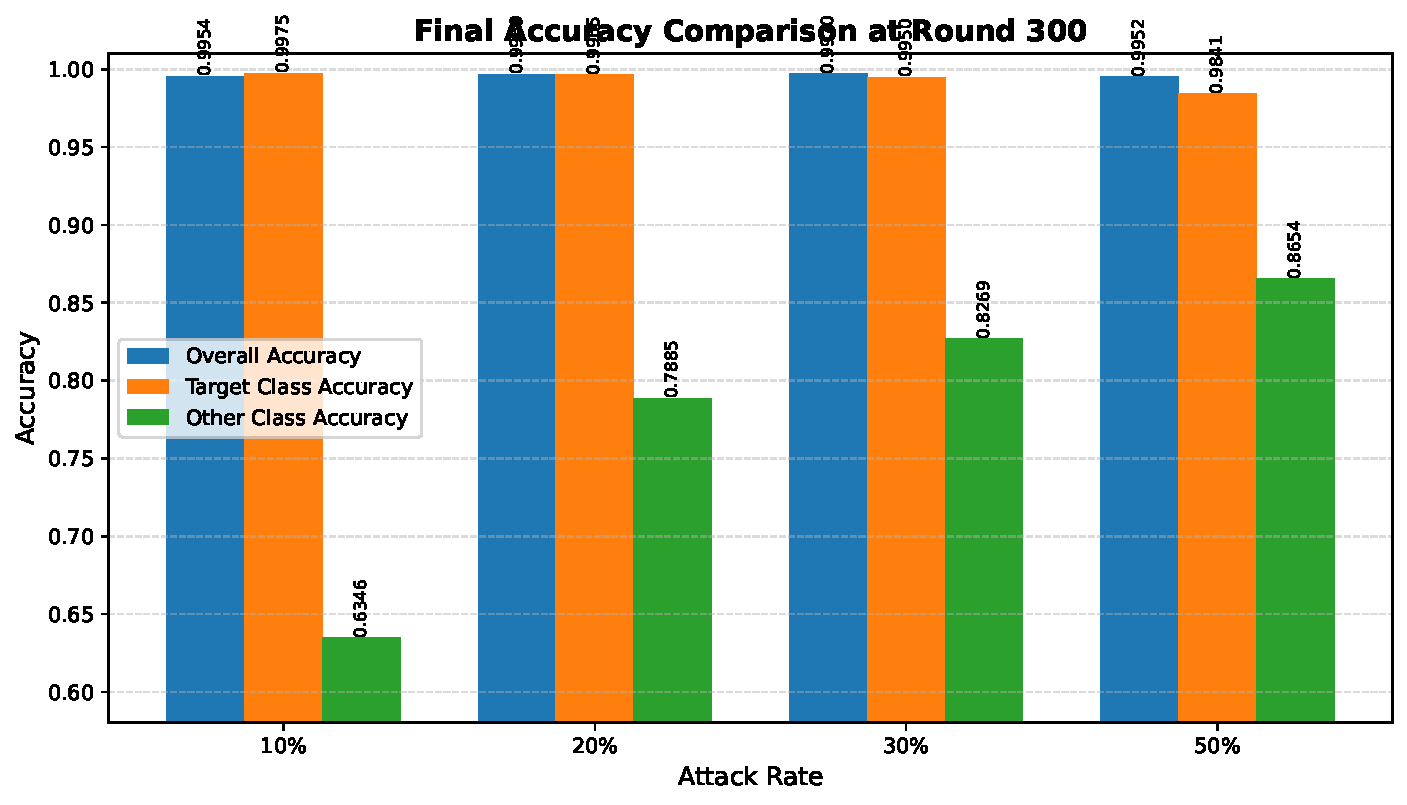
\includegraphics[width=0.47\textwidth]{fig_noniid_targeted_kdd_final_acc.pdf}}
\caption{KDDCup99 non-IID targeted attack results. The target-class trajectory remains high through training, and the round-300 comparison shows that overall and target-class accuracy stay stable even as the malicious-client fraction increases.}
\label{fig:res-noniid-targeted-kdd-dynamics}
\end{figure}

%=====================================================================
\section{IID Partition, Untargeted Attacks}
\label{sec:res-IID-untarg}

The IID rows are included mostly as a sanity-check baseline. With IID partitions the honest clients are statistically very close to one another, which means the distribution of FIP scores in any given round is comparatively tight, and detection should be the easiest setting we will see.

\subsection{MNIST}
\label{sec:res-IID-untarg-mnist}

\begin{table}[H]
\centering
\caption{MNIST, IID partition, untargeted label-flipping attack.}
\label{tab:res-IID-untarg-mnist}
\begin{tabular}{@{}cccccc@{}}
\toprule
\textbf{AR} & \textbf{ACC (\%)} & \textbf{$T_{\text{acc}}$ (\%)} & \textbf{$O_{\text{acc}}$ (\%)} & \textbf{TPR} & \textbf{FPR} \\
\midrule
10\% & 91.49 & 97.51 & 90.40 & 1.00 & 0.00 \\
20\% & 91.50 & 97.51 & 90.39 & 1.00 & 0.00 \\
30\% & 91.33 & 97.42 & 90.28 & 1.00 & 0.00 \\
50\% & 91.32 & 97.42 & 90.22 & 1.00 & 0.00 \\
\bottomrule
\end{tabular}
\end{table}

\subsection{KDDCup99}
\label{sec:res-IID-untarg-kdd}

\begin{table}[H]
\centering
\caption{KDDCup99, IID partition, untargeted label-flipping attack.}
\label{tab:res-IID-untarg-kdd}
\begin{tabular}{@{}cccccc@{}}
\toprule
\textbf{AR} & \textbf{ACC (\%)} & \textbf{$T_{\text{acc}}$ (\%)} & \textbf{$O_{\text{acc}}$ (\%)} & \textbf{TPR} & \textbf{FPR} \\
\midrule
10\% & 99.74 & 99.60 & 85.58 & 1.00 & 0.00 \\
20\% & 99.73 & 99.55 & 85.58 & 1.00 & 0.00 \\
30\% & 99.75 & 99.60 & 85.58 & 1.00 & 0.00 \\
50\% & 99.73 & 99.55 & 85.58 & 1.00 & 0.00 \\
\bottomrule
\end{tabular}
\end{table}

\paragraph{Observations.} In the IID untargeted setting, detection is essentially exact on both datasets --- every row reports $\mathrm{TPR}=1.00$ together with $\mathrm{FPR}=0.00$. The MNIST ACC moves by less than $0.2$ percentage points across the whole attack-rate sweep, and on KDDCup99 the ACC, $T_{\text{acc}}$, and $O_{\text{acc}}$ values together vary by at most $0.05$ percentage points.

\begin{figure}[!htbp]
\centering
\subfigure[MNIST ACC trajectory]{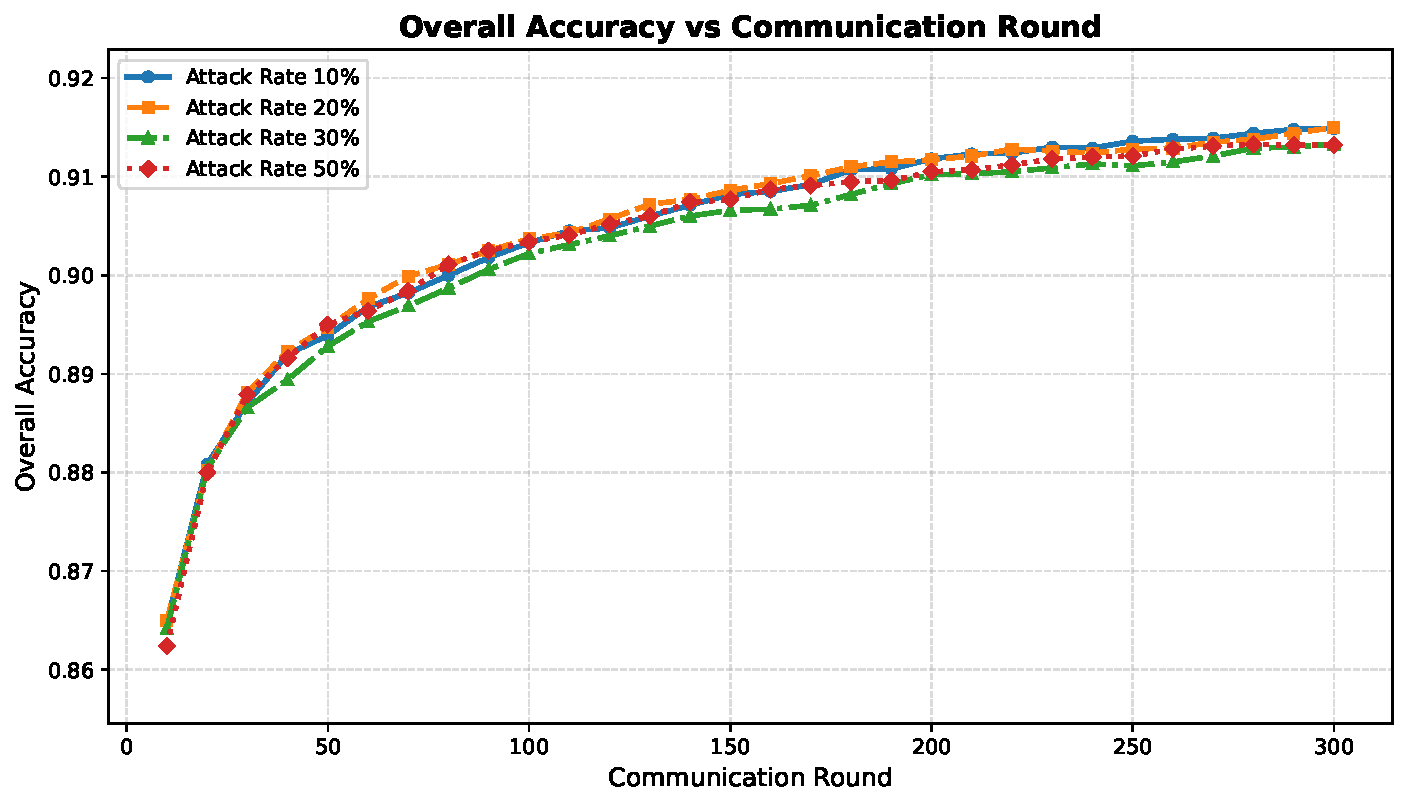
\includegraphics[width=0.47\textwidth]{fig_iid_untargeted_mnist_acc.pdf}}
\hfill
\subfigure[KDDCup99 ACC trajectory]{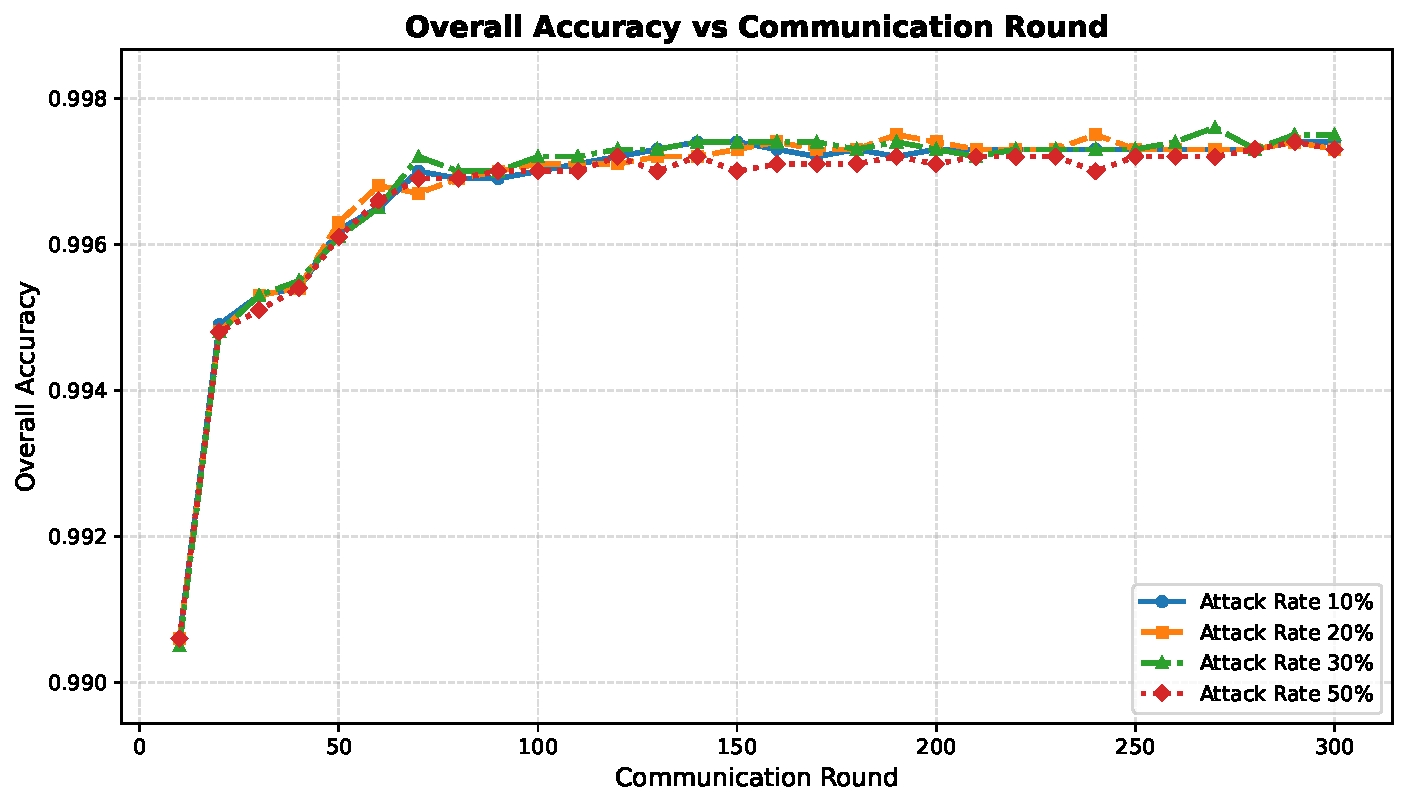
\includegraphics[width=0.47\textwidth]{fig_iid_untargeted_kdd_acc.pdf}}
\vspace{0.4em}
\subfigure[MNIST malicious-client TPR]{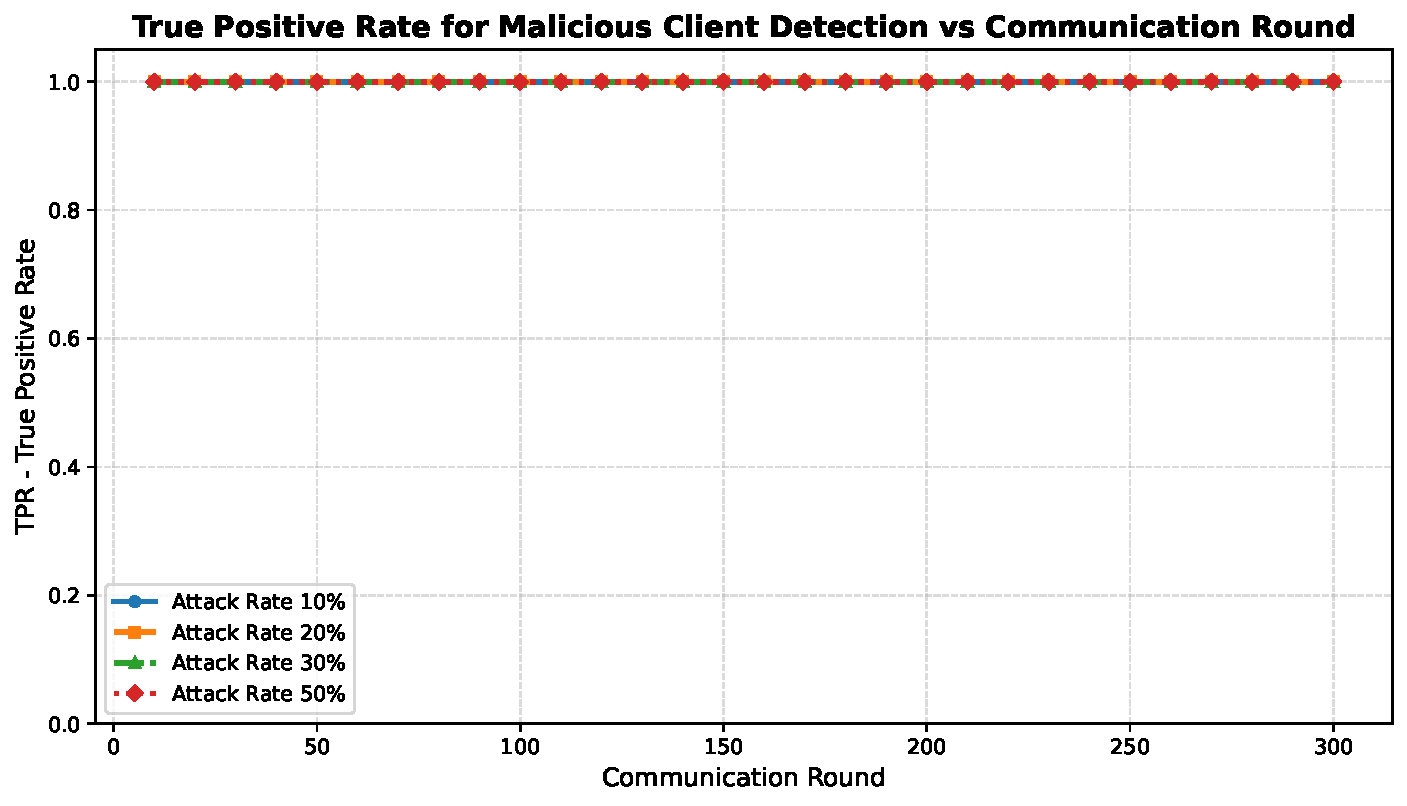
\includegraphics[width=0.47\textwidth]{fig_iid_untargeted_mnist_tpr.pdf}}
\hfill
\subfigure[KDDCup99 malicious-client TPR]{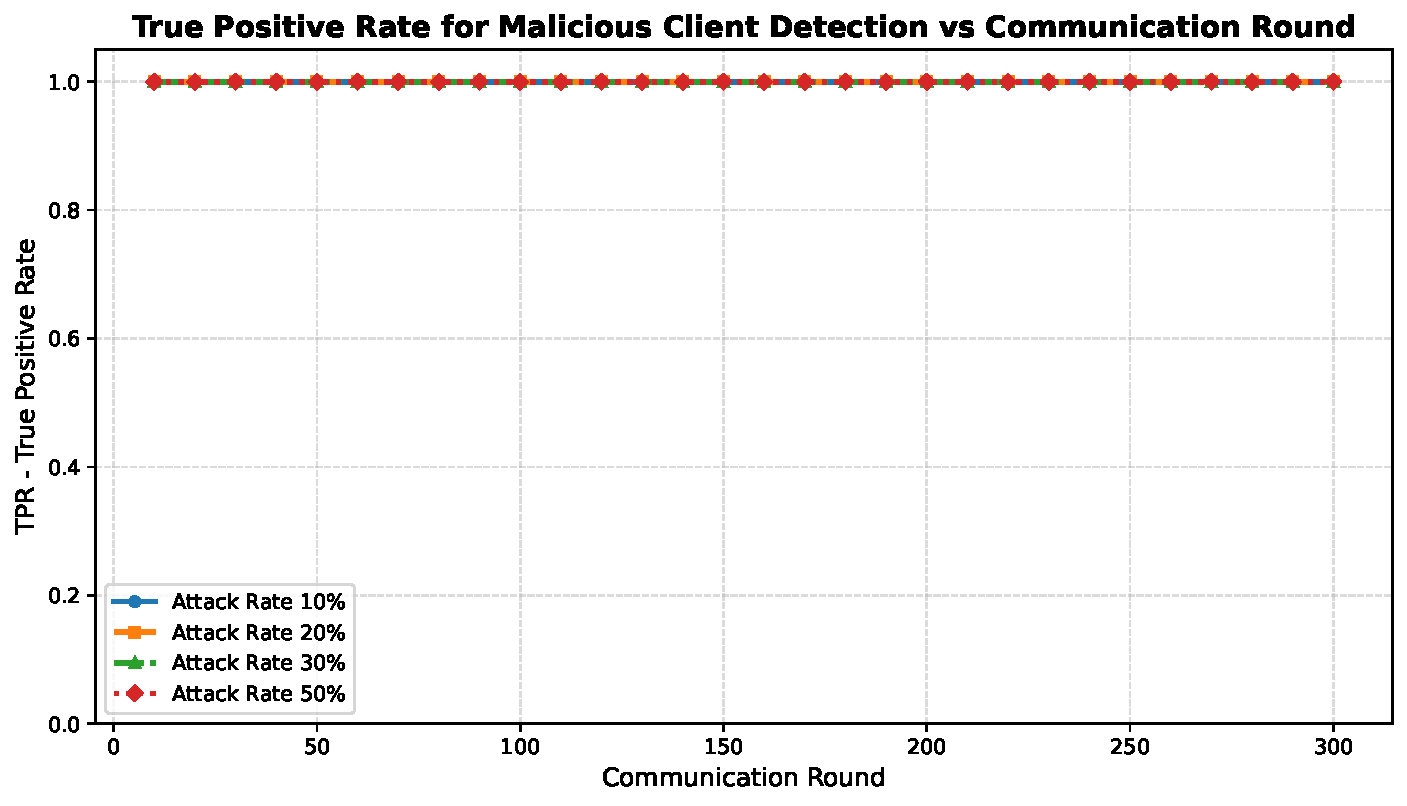
\includegraphics[width=0.47\textwidth]{fig_iid_untargeted_kdd_tpr.pdf}}
\caption{IID untargeted attack dynamics over 300 communication rounds. Both datasets show stable convergence, and the audit maintains perfect malicious-client detection without false positives at the reported final round.}
\label{fig:res-iid-untargeted-dynamics}
\end{figure}

%=====================================================================
\section{IID Partition, Targeted Attacks}
\label{sec:res-IID-targ}

\subsection{MNIST}
\label{sec:res-IID-targ-mnist}

\begin{table}[H]
\centering
\caption{MNIST, IID partition, targeted label-flipping attack $(c_s=0,c_t=7)$.}
\label{tab:res-IID-targ-mnist}
\begin{tabular}{@{}cccccc@{}}
\toprule
\textbf{AR} & \textbf{ACC (\%)} & \textbf{$T_{\text{acc}}$ (\%)} & \textbf{$O_{\text{acc}}$ (\%)} & \textbf{TPR} & \textbf{FPR} \\
\midrule
10\% & 91.62 & 97.51 & 90.57 & 1.00 & 0.00 \\
20\% & 91.42 & 97.42 & 90.35 & 1.00 & 0.00 \\
30\% & 91.32 & 97.42 & 90.22 & 1.00 & 0.00 \\
50\% & 91.43 & 97.42 & 90.35 & 1.00 & 0.00 \\
\bottomrule
\end{tabular}
\end{table}

\subsection{KDDCup99}
\label{sec:res-IID-targ-kdd}

\begin{table}[H]
\centering
\caption{KDDCup99, IID partition, targeted label-flipping attack.}
\label{tab:res-IID-targ-kdd}
\begin{tabular}{@{}cccccc@{}}
\toprule
\textbf{AR} & \textbf{ACC (\%)} & \textbf{$T_{\text{acc}}$ (\%)} & \textbf{$O_{\text{acc}}$ (\%)} & \textbf{TPR} & \textbf{FPR} \\
\midrule
10\% & 99.73 & 99.60 & 84.62 & 1.00 & 0.00 \\
20\% & 99.73 & 99.55 & 85.58 & 1.00 & 0.00 \\
30\% & 99.72 & 99.50 & 85.58 & 1.00 & 0.00 \\
50\% & 99.73 & 99.55 & 85.58 & 1.00 & 0.00 \\
\bottomrule
\end{tabular}
\end{table}

\paragraph{Observations.} The IID targeted case lines up cleanly with the IID untargeted one. Detection stays perfect, false rejections never happen, and the target-class accuracy stays flat across all attack rates. MNIST holds $T_{\text{acc}}\ge97.42\%$ across the table, and KDDCup99 keeps ACC in the $99.72\%$--$99.73\%$ band with $T_{\text{acc}}\ge99.50\%$ on every row.

\begin{figure}[H]
\centering
\subfigure[MNIST target-class accuracy]{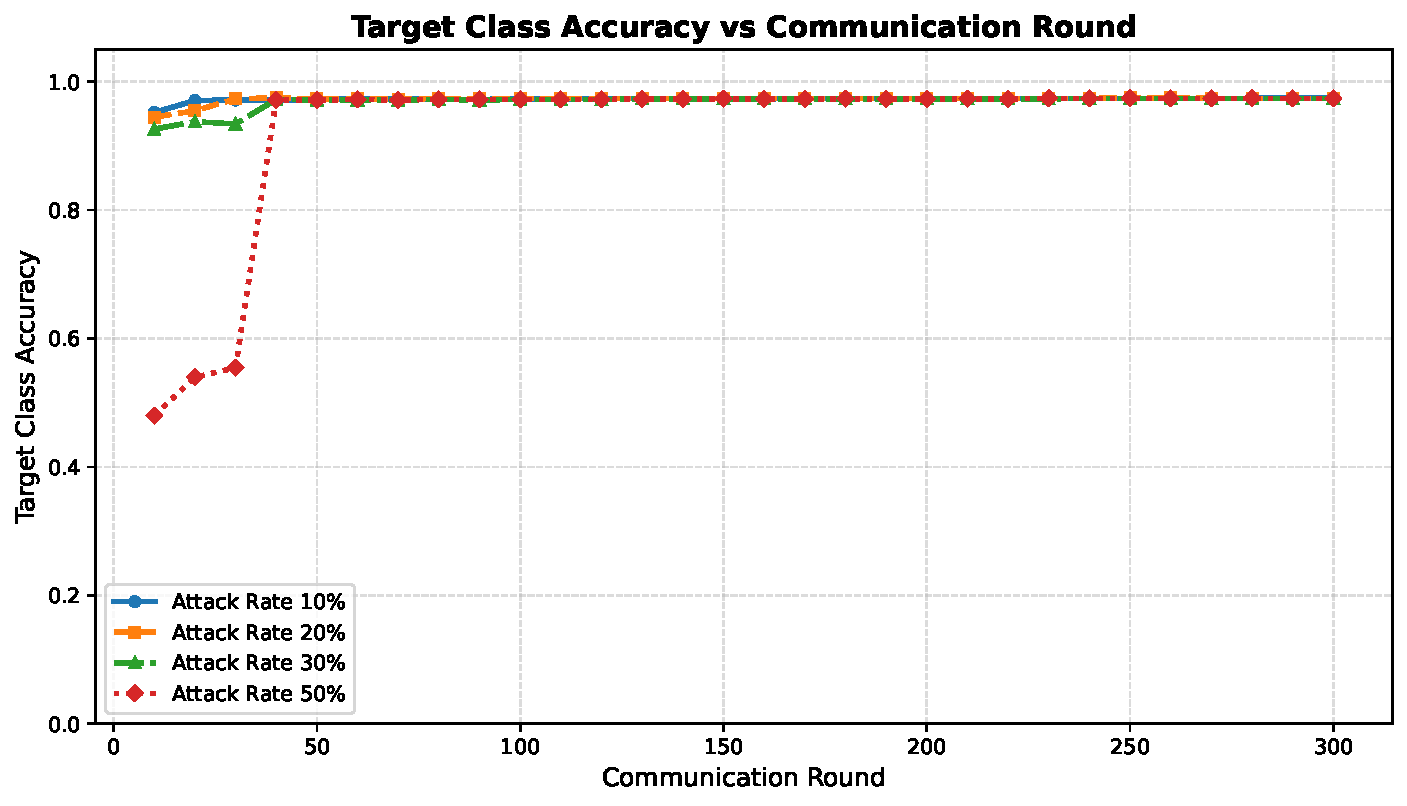
\includegraphics[width=0.47\textwidth]{fig_iid_targeted_mnist_tacc.pdf}}
\hfill
\subfigure[KDDCup99 target-class accuracy]{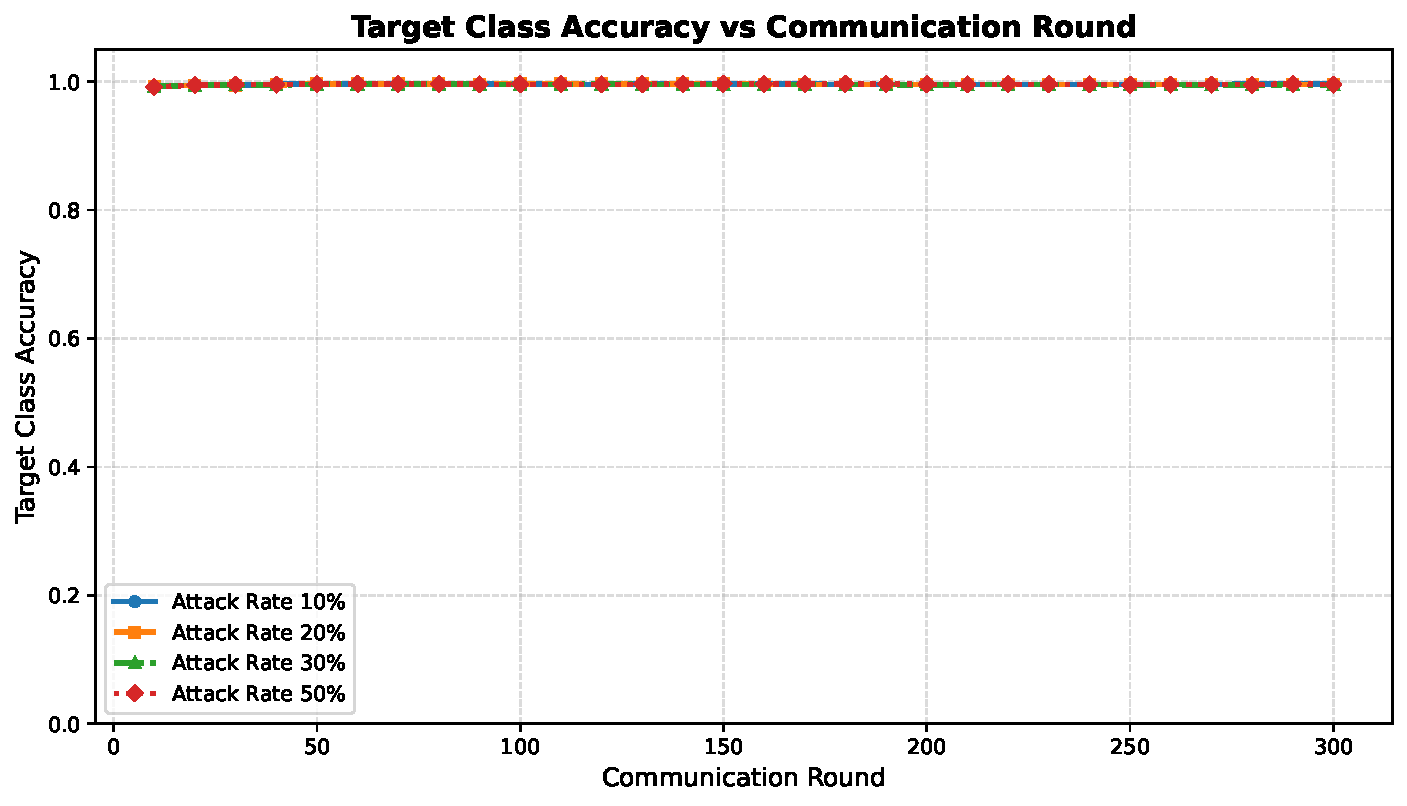
\includegraphics[width=0.47\textwidth]{fig_iid_targeted_kdd_tacc.pdf}}
\caption{IID targeted attack target-class accuracy over 300 communication rounds. In both datasets, the target class recovers to a stable high-accuracy regime by the final round.}
\label{fig:res-iid-targeted-dynamics}
\end{figure}

%=====================================================================
\section{Aggregate Findings Across the Grid}
\label{sec:res-aggregate}

Stepping back from the individual tables, the grid as a whole supports three conclusions. First, every completed row reports $\mathrm{TPR}=1.00$, including the $50\%$ malicious-client cases on both datasets. Second, false rejection only shows up under the heaviest non-IID untargeted load --- exactly the regime where the honest gradients are already pulled apart by label skew --- and even there ACC remains numerically stable. Third, targeted attacks are caught just as reliably as untargeted ones, which suggests that a one-dimensional FIP score against the trusted reference is genuinely sufficient for the poisoning regimes evaluated here. Chapter~\ref{Comparison:chap:chap8} puts these numbers next to the auditor-based baseline.
